\chapter{Kravspecifikation}
\label{ch:kravspecikikation}
Kravspecifikationen er udarbejdet i begyndelsen af projektforløbet og omfatter use cases, ikke funktionelle krav samt kvalitets faktorer. For den fulde kravspecifikation, henvises der til dokumentions dokumentet.

\subsection{Overordnede krav til systemet}
Systemet skal indeholde én til flere sensorer samt en til flere aktuatorer. Endvidere skal systemet indeholde et kontrolinterfacet og et styringsmodul. Kontrolinterfacet fungerer som brugergrænesflade og har kontakt til en ekstern database.

\subsection{Funktionelle krav}
Systemets funktioner er beskrevet vha. Use Cases. Før use cases udfærdiges nedskrives systemets akører. Der laves hertil en beskrivelse af deres funktion samt ansvar i systemet. I hver Use case er der en beskrivelse af en enkelt funktionalitet systemet skal have.
\begin{figure}[H]
\centering
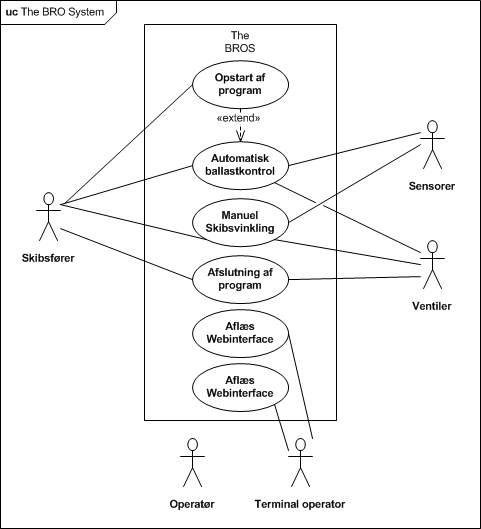
\includegraphics[width=0.6\textwidth]{billeder/UCDBROS}
\caption{Use Case Diagram for BROS}
\label{fig:UCDBROS}
\end{figure}
Der er også beskrevet alternative hændelser, såfremt hældelsesforløbet ikke forløber som planlagt. Alle use cases har fulgt samme fremgangsprocedure. Se kravspecifikationsdokumentet for alle systemets Use Cases. På \textit{Figur~\ref{fig:UCDBROS}} ses Use Cases for systemet.\\
Når systemet startes op første gange anvendes Opstart af Program(Use Case 1). Når systemet er startet op kan brugeren vælge mellem Automatisk ballastkontrol (Use Case 2) eller Manuel Skibsvinkling (Use Case 3). Hvis brugeren vil deaktivere systemet kan han afslutte programmet (Use Case 4). En Terminaloperator kan tilgå databaseinformationen via et Webinterface(Use Case 5 og 6).


\subsection{Ikke funktionelle krav}
I dette afsnit beskrives krav til tolerancer og andre krav der ikke er use case specifikke. Nedenfor er noteret nogle ikke funktionelle krav:
\begin{itemize}
\item Sensorer:
\begin{itemize}
\item[$\diamond$] Hældningssensor:\\
Hældningssensor måler skibets hældning i forhold til vandret i området -7.5 til 7.5 grader, med en nøjaftighed på 0.5 grader.\\
\item[$\diamond$] Ballasttank\\
Vandniveauet i ballasttanken skal måles fra 0-100\% med en nøjagtighed på $\pm$2.5\%-point.
\end{itemize}
\item Alarmer:
\begin{itemize}
\item[$\diamond$]Vandniveauet i ballasttanke bliver mere end 70\%.
\item[$\diamond$]Hældning på skibet bliver større end $\pm$5 grader.
\item[$\diamond$]Mistet eller ingen forbindelse internt i systemet.
\item[$\diamond$]Mistet eller ingen forbindelse til ekstern database.
\end{itemize}
\end{itemize}
\subsection{Krav til udvinklingsprocess og teknologi}
Projektforløbet skal følge V-modellen. SCRUM skal bruges i projektstyringsprocessen til at give overblik over projektets arbejdsopgaver. SCRUMmaster og projektleder uddeles til gruppemedlemmer.\\
Til dokumentation skal der bruges SysML diagrammer til at beskrive systemet overordnet og i detaljer.\\
Programmeringen til systemets embedded enheder, Styringsmodulet og Vandballasttankenhederne, anvendes C. Til kontrolinterfaces og databasen anvendes C++. Til Databaselagring anvendes mySQL. Webinterfacet skal skrives i php og HTML 5.

\subsection{Krav til grænseflader}
Kommunikationen mellem kontrolinterfacet og styringsmodulet skal følge UART protokollen. Det kan kun tilkobles ét kontrolinterface og ét styringsmodul.\\
Til styringsmodulet tilkobles én sensor samt to vandballasttankenheder via. I2C protokollen.\\
På kontrolinterfacet skal alt funktionaliteten være indbygget i brugergrænsefladen. Det skal være muligt at skifte mellem automatisk ballastkontrol og manuel skibsvinkling. \fxnote{Lund skal lige beskrive resten af GUI'en}

\subsection{Krav til kvalitet}
For at sikre kvaliteten af vores produkt har vi valgt at opstille en række kvalitetsfaktorer. Det er meget vigtigt for vores system at det er pålideligt, sikkert og Effektivt. Pålideligheden skyldes at systemet kan risikere at være fatalt for et skib, hvis der sker en fejl. Systemet skal være sikkert da det er en kritisk komponent. Endvidere skal systemet være effektivt da det ikke må sløve lastning og losningsprocessen.\\
Krav til Brugervenlighed og vedligeholdsesvenlighed er middelvægtet, da brugerens anvendelse af systemet skal hjælpe til processen og ikke gøre den yderligere kompliceret. Systemet skal kunne vedligeholdes af en tilkaldt operatør.\\
